%!TEX root = ../main.tex

\chapter{Kravspecifikation}

\RevisionsTabel{Kravspecifikation}{
Alle	& X 	& XX-XX-XXXX  \\
}

%Aktører
\section{Aktører}
%!TEX root = ../Main.tex

I dette afsnit beskrives aktører og deres rolle i systemet. I figur~\ref{fig:actordiagram} ses aktørdiagram, som beskriver alle aktører og deres forhold til systemet.
\begin{figure}
	\centering
	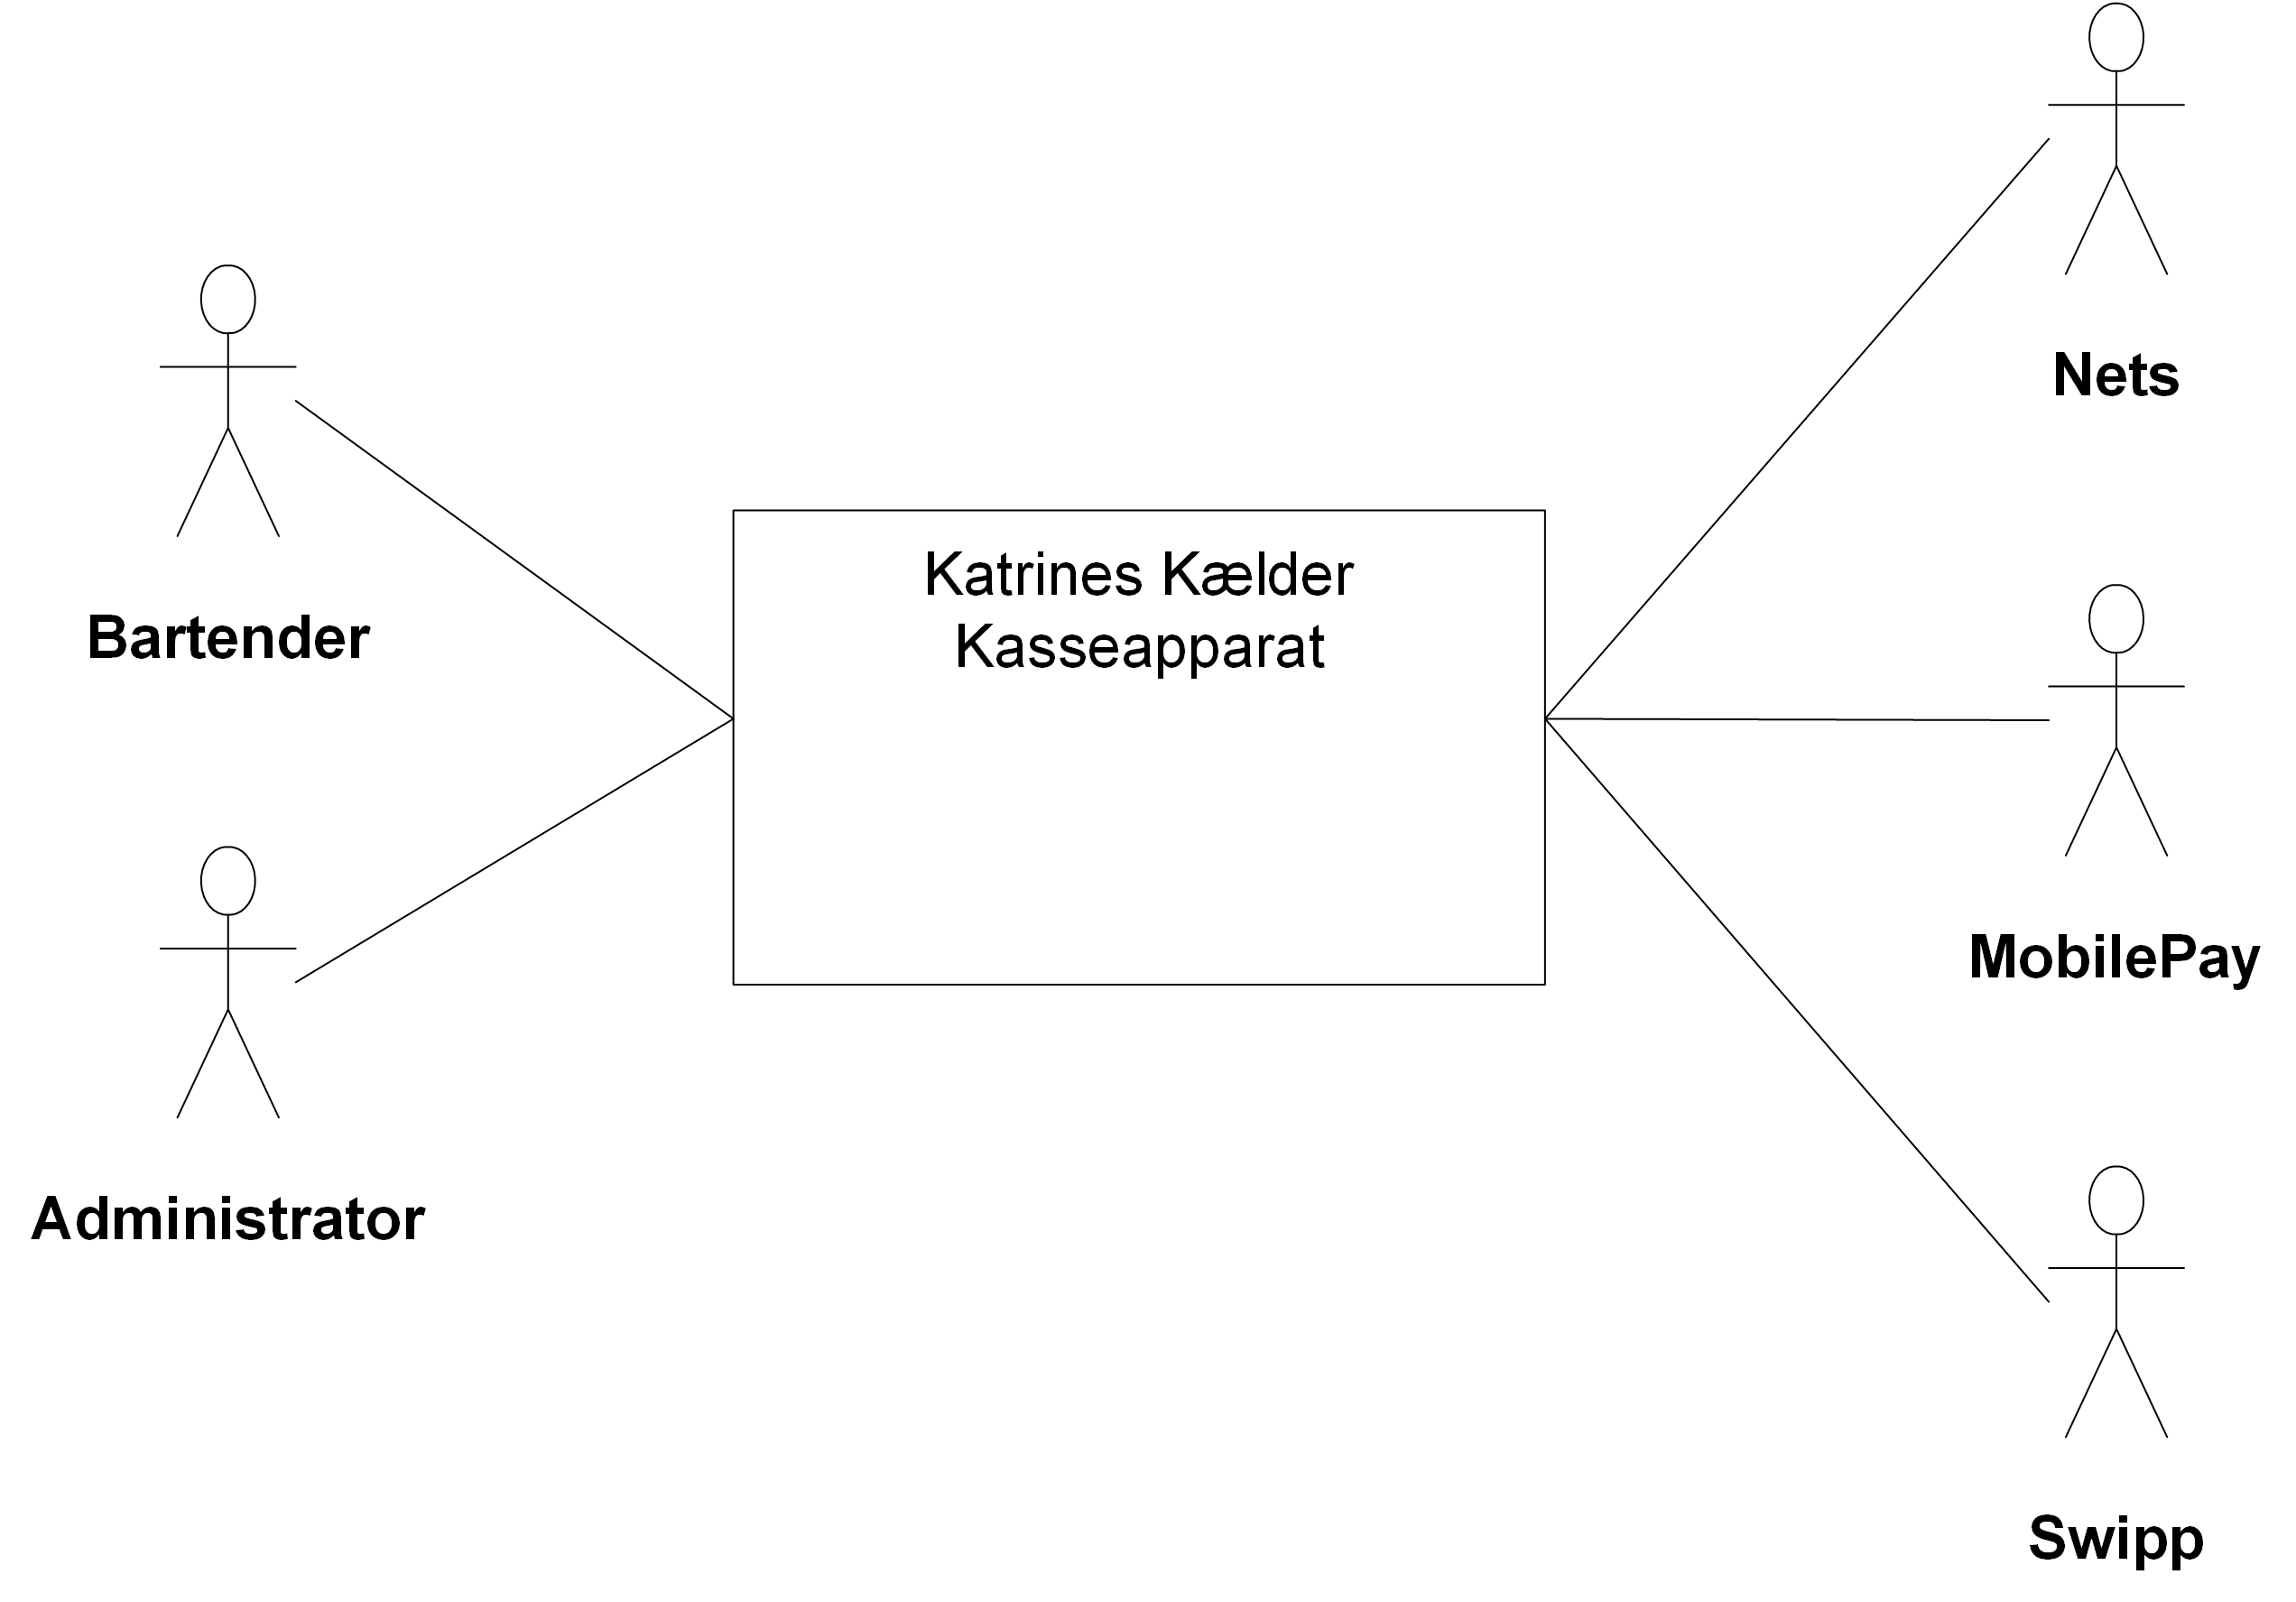
\includegraphics[width=0.8\textwidth]{Kravspecifikation/Actor/Actor.png}
	\caption{Aktør-kontekst diagram}
	\label{fig:actordiagram}
\end{figure}

\newpage
\subsection{Bartender}
\begin{usecase}
\title{Aktørnavn}{Bartender} 
\field{Type:}{Primær}
\field{Beskrivelse:}{\textit{Bartender} er den primære bruger af systemet. Aktøren skal stå for servicering af kunden og opsætning af en evt. transaktion gennem systemet.}
\end{usecase}

\subsection{Admin}
\begin{usecase}
\title{Aktørnavn}{Admin} 
\field{Type:}{Primær}
\field{Beskrivelse:}{\textit{Admin} skal stå for logistikken (priser, varelager osv.) gennem systemet.}
\end{usecase}

\subsection{Nets}
\begin{usecase}
\title{Aktørnavn}{Nets} 
\field{Type:}{Sekundær}
\field{Beskrivelse:}{\textit{Nets} er leverandøren af Dankort-systemet. Betalingsløsningen er en af systemets primære betalingsløsninger.}
\end{usecase}

\subsection{MobilePay}
\begin{usecase}
\title{Aktørnavn}{MobilePay} 
\field{Type:}{Sekundær}
\field{Beskrivelse:}{\textit{MobilePay} er en betalingsløsning, som leveres af Danske Bank.}
\end{usecase}

\subsection{Swipp}
\begin{usecase}
\title{Aktørnavn}{Swipp} 
\field{Type:}{Sekundær}
\field{Beskrivelse:}{\textit{Swipp} er en betalingsløsning, som leveres af Nordea, Nykredit, Sydbank, Jyske Bank, Arbejdernes Landsbank, Spar Nord Bank og Lokale Pengeinstitutter.}
\end{usecase}

%Use Cases
\newpage
\section{Use Cases}
%	Indledning
I dette afsnit ses de forskellige Use cases. På billede ---- ses et Use case-diagram, som viser en simpel repræsentation af 
\newpage

%	#1 -------
\newpage
%!TEX root = ../../main.tex

\subsection*{Use case 1}
I denne use case ser vi hvor et kontant salg bliver foretaget
\begin{usecase}{1}

\title{ Kontant Salg } 

\field{Mål:}{ At sælge drikkevarer mod kontant betaling }

\field{Initieret af:}{ Bartender }

\field{Aktører:}{ Bartender }

\field{Samtidige forekomster:}{1}

%Preconditions: What must be true on start and worth telling the reader?
\field{Prækondition:}{System skal være tændt og klar}

%Postconditions: What must be true on successful completion and worth telling the reader
\field{Postkondition:}{ Et kontant salg er foretaget }

%Main Success Scenario: A typical, unconditional happy path scenario of success.
\scenario{Hovedscenarie:}{
	\item Bartender vælger drink(s)/pris(er) på systemets touchskærm
	\item Bartender trykker "Total"	
	\item Den samlede pris udregnes
	\item Bartender trykker "Kontant" og skuffen åbnes
	\item Bartender modtager betaling fra kunden
	[Extension 1.1: Kontanter ikke modtaget]
	\item Købet er afsluttet
}


%Extensions: Alternate scenarios of success or failure.
\scenario{Extension 1.1: Kontanter ikke modtaget:}{
		\item Bartender trykker annuller køb
		\item Bartender lukker skuffen
		\item Systemet er klar til næste kunde
}


\end{usecase}


%!TEX root = ../../main.tex

\subsection*{Use case 1}
I denne use case -----
\begin{usecase}

\addtitle{Use Case 2}{ Udskriv Kundebon } 

\addfield{Mål:}{ Systemet får udskrevet en bon med kundens køb på }

\addfield{Initieret af:}{ Bartender }

\addfield{Aktører:}{ Bartender (Primær) }

\addfield{Samtidige forekomster:}{1}

%Preconditions: What must be true on start and worth telling the reader?
\addfield{Prækondition:}{Use Case 1 er gennemført}

%Postconditions: What must be true on successful completion and worth telling the reader
\addfield{Postkondition:}{Kunden (baretender?) modtager bon med køb på }

%Main Success Scenario: A typical, unconditional happy path scenario of success.
\addscenario{Hovedscenarie:}{
	\item Bartender har valgt at der skal udskrives bon (på GUI?)
	\item En dialogbox popper op og bartender bekræfter ønske af bon	
	\item printer udskriver bon  [Ext 1: Der er ikke mere papir]
	\item Bartender udleverer bon til kunde [Ext 2: Kunde er gået]	
}

%Extensions: Alternate scenarios of success or failure.
\addscenario{Udvidelser:}{
	\item[Ex.1] Der er ikke mere papir
		\begin{enumerate}
		\item[1.] Printer stopper. Dialogbox popper op med besked "Fyld papir på printer"
		\item[2.] Bartender fylder papir på printer.
		\item[3.] Der trykkes på 'OK' og fortsættes fra punkt 3
		\end{enumerate}
	\item[Ex.2] Kunde er gået
		\begin{enumerate}
			\item[1.] Bartender smider bon ud
		\end{enumerate}
}


\end{usecase}




%	#Ikke fully dressed Use cases
\newpage
\section{Ikke fully dressed use cases}

\subsubsection*{Use Case 4 - Dankort Salg}
skal beskrive forløbet for et salg når kasseapparatet interagerer med dankort automaten.

\subsubsection*{Use Case 5 - Medarbejder Salg}
Heri beskrives forløbet for salg til en medarbejder der opnår rabat.

\subsubsection*{Use Case 6 - Indtastning af lager varer}
Til lagerstyrings delen af produktet skal der være mulighed for at indtaste vare i systemet når de ankommer/bestilles.

\subsubsection*{Use Case 7 - Admin login}
For at kunne ændre priser, indsætte nye varer osv. skal der kunne logges ind på en administrationsdel af systemet således at ikke alle og enhver kan gøre dette.

\subsubsection*{Use Case 8 - Fjern lagervarer}
Når der hentes varer på lageret skal disse kunne tjekkes ud af systemet.

\subsubsection*{Use Case 9 - Tilføj varer til kasseapparat}
Det skal være muligt at tilføje en varer til kasseapparatet denne use case kræver at admin login use casen er udført.

\subsubsection*{Use Case 10 - Rediger varer i kasseapparat}
Det skal være muligt at ændre en varers pris og navn osv. denne use case kræver admin login use casen er udført.

\subsubsection*{Use Case 11 - Fjern varer fra kasseapparat}
Det skal være muligt at fjerne drinks fra systemet hvis de f.eks. ikke længere bliver serveret. denne use case kræver admin login use casen er udført.

\subsubsection*{Use Case 12 - Vis Statistik over salg}
Der skal kunne generes en statistik over de varer der er blevet solgt gerne i detaljer der specifikt beskriver hvilke drinks der er solgt.

\subsubsection*{Use Case 13 - Scan varer til lager}
Der skal kunne bruges et apparat der kan scanne varer ind i lager systemet. 

%   #Ikke funktionelle krav
\newpage
\section{Ikke Funktionelle Krav}
MoSCoW metoden er blev brugt til at afgrænse produktet og identificere de vigtigste egenskaber. Det giver en opdeling således:

\subsection{Must}
\begin{itemize}
\item have en GUI der kan betjenes med en touchskærm.
\item interagere med betalingskort, systemet skal kunne sende en betaling til betalingsterminalen.
\item have en printer der kan printe boner.
\item have en kontantskuffe der kan åbnes via systemet.
\item logge alt salg.
\item have en backup af salgslog.
\end{itemize}

\subsection{Should}
\begin{itemize}
\item tilføje nye varer til GUI.
\item ændre priser på varer.
\item fjerne varer.
\item have mulighed for lagerstyring.
\item have et administrator login til opsætning.
\end{itemize}

\subsection{Could}
\begin{itemize}
\item have farvekode på forskellige varer.
\item bruge MobilePay til at modtage betaling.
\item bruge Swipp til at modtage betaling.
\item have en statistik af solgte varer.
\item have en stregkodescanner til brug ved lagerstyring.
\end{itemize}

\subsection{Won't}
\begin{itemize}
\item have brugere til individuelle bartenderer.
\end{itemize}

%	#Skitse over interface
\section{Systemets grænseflader}
Dette afsnit vil beskrive systemet grænseflader.

\subsection{Grænseflader til person aktører}
Systemet har to person grænseflader: Bartender og Admin.
\newline\newline
Bartender kan vha. brugergrænsefladen:
\begin{itemize}
	\item Udføre salg
	\item Tage imod betaling
\end{itemize}

Admin kan vha. WebAPI'et:
\begin{itemize}
	\item Oprette, redigere og slette produkter.
\end{itemize}

\subsection{Grænseflader til eksterne system aktører}
Systemet har tre eksterne system aktører: Nets, MobilePay og Swipp. Nets -- altså Dankort -- har været første prioritet i forhold til betalingsudbydere. Da systemet stadig i udviklingsfasen, hvor Dankort skal implementeres vil Nets kun blive beskrevet i dette afsnit.
\newline\newline
Nets er udbyderen af Dankort systemet. Systemet skal interagere med den API, som er stillet til rådighed fra Nets. Selve API'en og interaktionen med systemet er ikke undersøgt nærmere. 

%\subsection{Grænseflader til hardware aktører}

%\subsection{Grænseflader til eksterne software aktører}
